\documentclass[12pt,letterpaper]{article}
\usepackage[utf8]{inputenc}
\usepackage[spanish]{babel}
\usepackage{graphicx}
\usepackage[left=2cm,right=2cm,top=2cm,bottom=2cm]{geometry}
\usepackage{graphicx} % figuras
% \usepackage{subfigure} % subfiguras
\usepackage{float} % para usar [H]
\usepackage{amsmath}
%\usepackage{txfonts}
\usepackage{stackrel} 
\usepackage{multirow}
\usepackage{enumerate} % enumerados
\renewcommand{\labelitemi}{$-$}
\renewcommand{\labelitemii}{$\cdot$}
% \author{}
% \title{Caratula}
\begin{document}

% Fancy Header and Footer
% \usepackage{fancyhdr}
% \pagestyle{fancy}
% \cfoot{}
% \rfoot{\thepage}
%

% \usepackage[hidelinks]{hyperref} % CREA HYPERVINCULOS EN INDICE

% \author{}
\title{Caratula}

\begin{titlepage}
\begin{center}
\large{UNIVERSIDAD PRIVADA-DE-TACNA}\\
\vspace*{-0.025in}
\begin{figure}[htb]
\begin{center}

\includegraphics[width=8cm]{./Imagenes/logo}
\end{center}
\end{figure}
\vspace*{0.15in}
INGENIERIA DE SISTEMAS  \\

\vspace*{0.5in}
\begin{large}
TITULO:\\
\end{large}

\vspace*{0.1in}
\begin{Large}
\textbf{INFORME DE LABORATORIO No 01}\\
\end{Large}

\vspace*{0.3in}
\begin{Large}
\textbf{CURSO:} \\
\end{Large}

\vspace*{0.1in}
\begin{large}
INTELIGENCIA DE NEGOCIOS\\
\end{large}

\vspace*{0.3in}
\begin{Large}
\textbf{DOCENTE(ING):} \\
\end{Large}

\vspace*{0.1in}
\begin{large}
 Patrick Cuadros Quiroga\\
\end{large}

\vspace*{0.2in}
\vspace*{0.1in}
\begin{large}
Estudiante: \\ 
Sharon Sosa Bedoya          (2016054460) \\
\end{large}
\end{center}

\end{titlepage}


\tableofcontents % INDICE
\thispagestyle{empty} % INDICE SIN NUMERO
\newpage
\setcounter{page}{1} % REINICIAR CONTADOR DE PAGINAS DESPUES DEL INDICE

\section{INFORMACIÓN GENERAL} 

\begin{itemize}
\subsection{Objetivos:}
	\item Generar todos los modelos fisicos de los diagramas entidad relación y modelo dimensional en bases de datos separadas en Microsoft SQL Server.
	\item Conocimientos básicos de administración de base de datos Microsoft SQL Server.
\subsection{Equipos, materiales, programas y recursos utilizados:}
	\item Windows 10 64bit: Pro, Enterprise o Education, con al menos 4GB de RAM.
	\item Base de datos AdventureWorksLT2016 o superior
	\item Tener los archivos de recursos del laboratorio.
	\item Microsoft SQL Server 2017 o superior

\end{itemize}

\section{PROCEDIMIENTO} 

\begin{itemize}
\subsection{Ejercicio 1: Envios}
	\subsubsection{Enunciado}

		\item El siguiente diagrama E / R simplificado describe el envío de mercancías. Los lotes pertenecientes a ciertos grupos se
envían a ciertos destinos en varios países a través de diferentes modos de transporte. Un cierto centro de costos es responsable de cada envío. La dimensión de tiempo consiste en mes y año.

	\begin{center}
	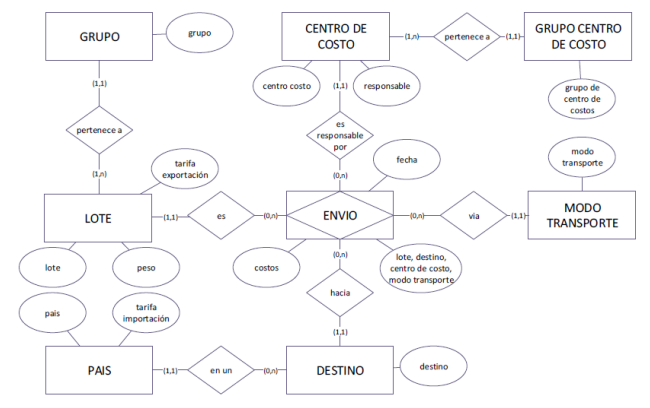
\includegraphics[width=14cm]{./Imagenes/ejercicio1}
	\end{center}

     \subsubsection{Modelo Dimensional }
	\begin{center}
	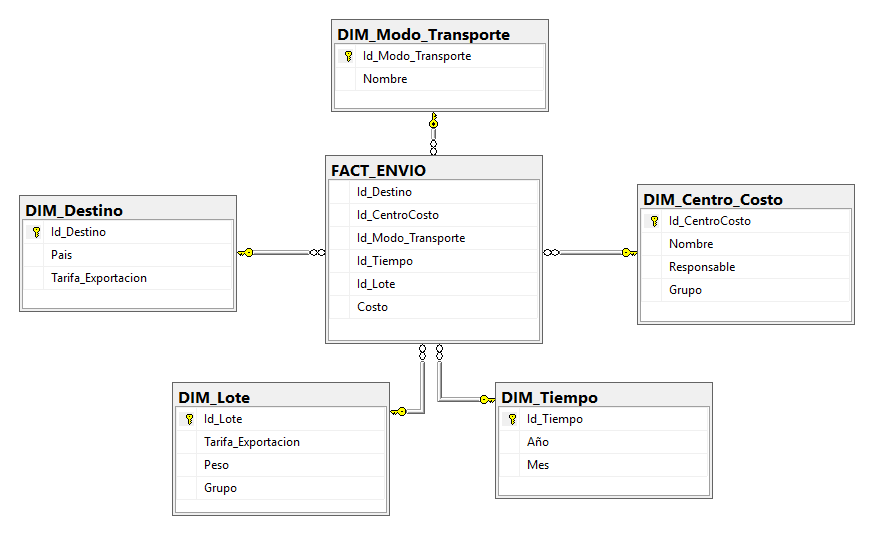
\includegraphics[width=14cm]{./Imagenes/ejercicio1_dimensional}
	\end{center}
   \subsubsection{Diagrama Físico }
	
	\begin{center}
	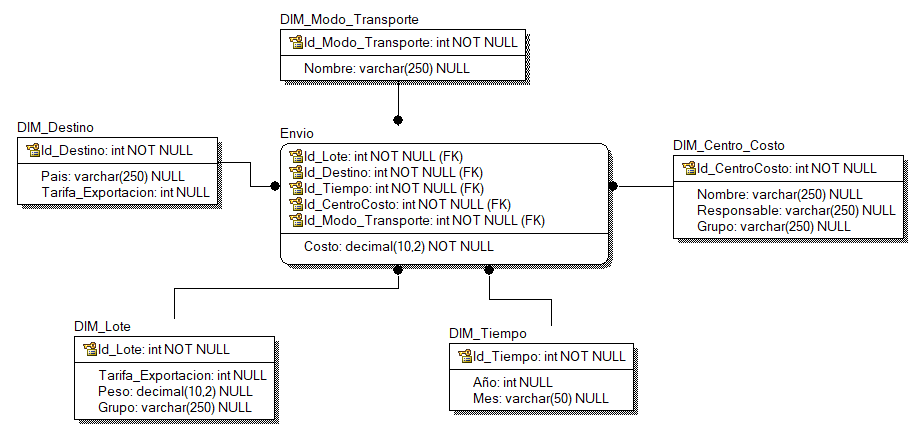
\includegraphics[width=14cm]{./Imagenes/ejercicio1_fisico}
	\end{center}

 \subsubsection{Script }
\begin{center}
	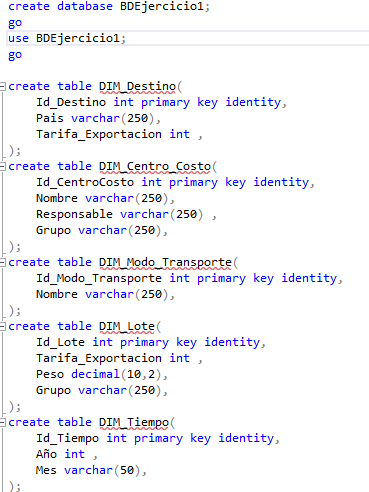
\includegraphics[width=8cm]{./Imagenes/ej1_script1}
	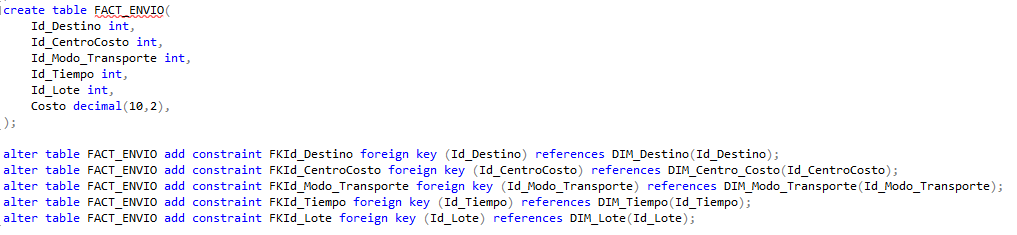
\includegraphics[width=14cm]{./Imagenes/ej1_script2}
	\end{center}


\subsection{Ejercicio 2: : Reservas de Viaje}

\subsubsection{Enunciado}

		\item En este esquema de E / R, un cliente (que es de cierto tipo) reserva un viaje en una agencia de viajes. La agencia de viajes trabaja para un determinado operador turístico. El viaje va a un destino determinado que pertenece a un país determinado.
La dimensión de tiempo consiste en mes, trimestre y año.

	\begin{center}
	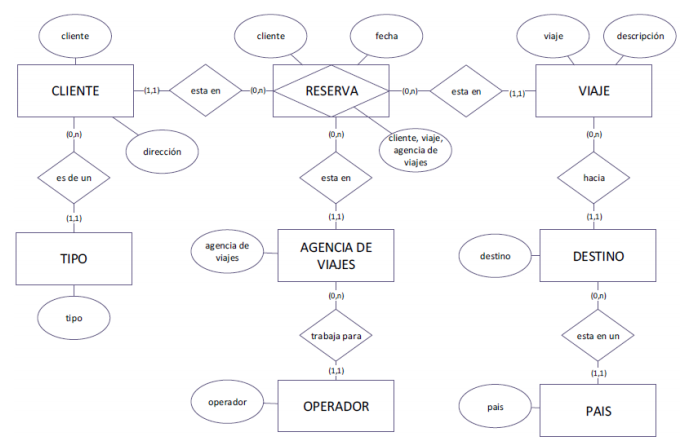
\includegraphics[width=14cm]{./Imagenes/ejercicio2}
	\end{center}

     \subsubsection{Modelo Dimensional }
	\begin{center}
	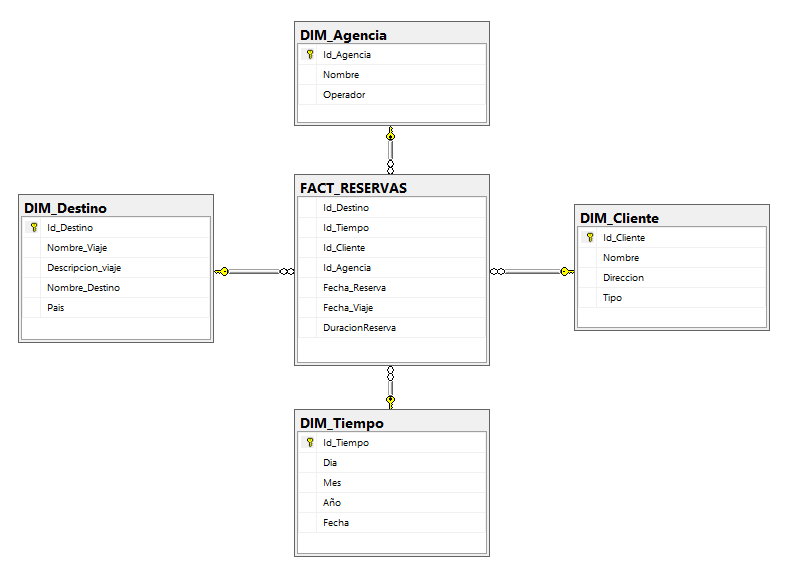
\includegraphics[width=14cm]{./Imagenes/ejercicio2_dimensional}
	\end{center}
   \subsubsection{Diagrama Físico }
	
	\begin{center}
	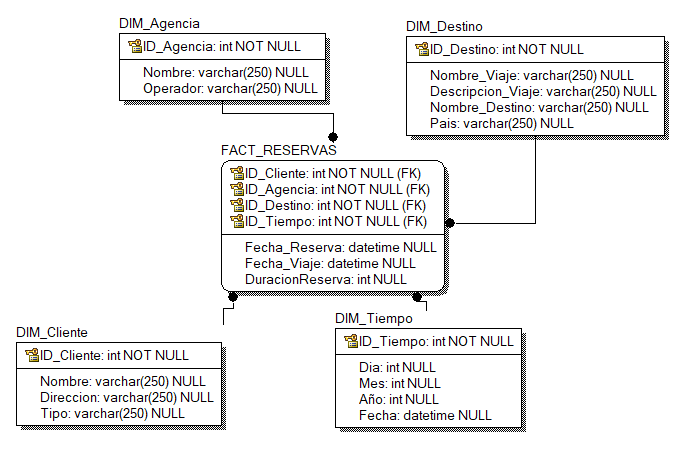
\includegraphics[width=14cm]{./Imagenes/ejercicio2_fisico}
	\end{center}

 \subsubsection{Script }
\begin{center}
	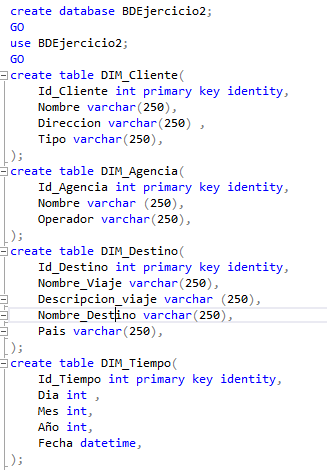
\includegraphics[width=8cm]{./Imagenes/ej2_script1}
	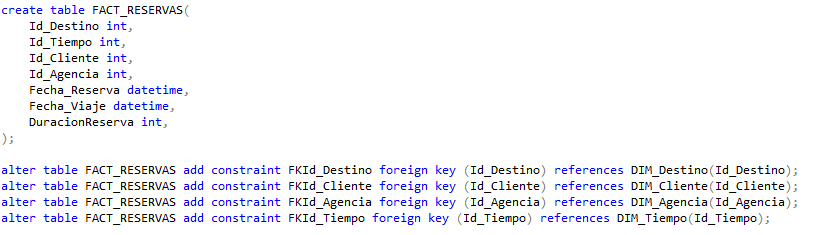
\includegraphics[width=14cm]{./Imagenes/ej2_script2}
	\end{center}

\subsection{Ejercicio 3: Gestión de proyectos}

\subsubsection{Enunciado}

		\item Este esquema E / R simplificado muestra un caso gestión del proyecto. El proyecto para un cliente se divide en varios paquetes de trabajo y siempre una persona es responsable de completar la tarea. Se cuida en un lugar determinado.
La dimensión de tiempo consiste de día, mes y año.

	\begin{center}
	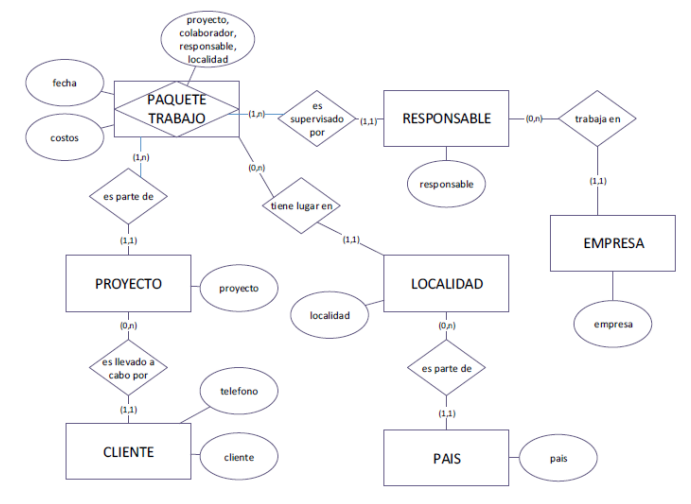
\includegraphics[width=14cm]{./Imagenes/ejercicio3}
	\end{center}

     \subsubsection{Modelo Dimensional }
	\begin{center}
	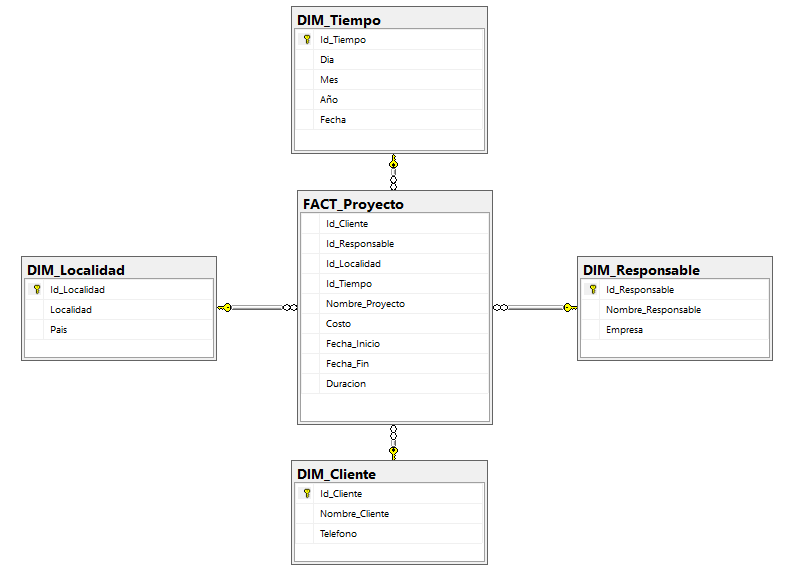
\includegraphics[width=14cm]{./Imagenes/ejercicio3_dimensional}
	\end{center}
   \subsubsection{Diagrama Físico }
	
	\begin{center}
	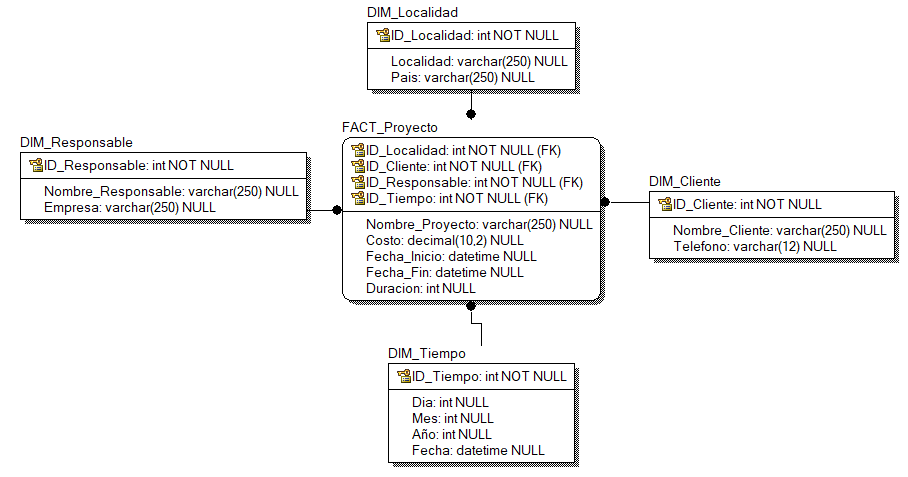
\includegraphics[width=14cm]{./Imagenes/ejercicio3_fisico}
	\end{center}

 \subsubsection{Script }
\begin{center}
	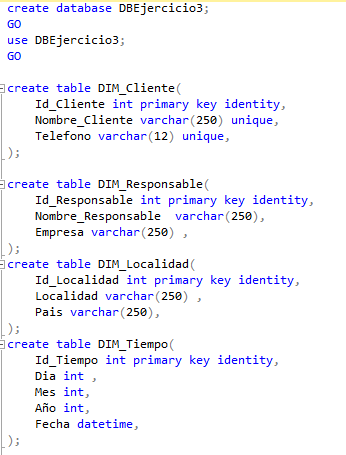
\includegraphics[width=8cm]{./Imagenes/ej3_script1}
	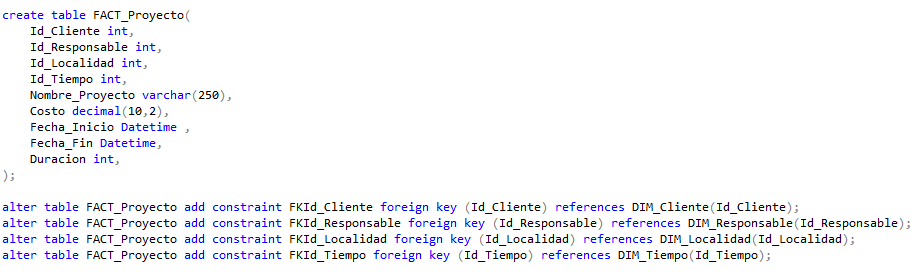
\includegraphics[width=14cm]{./Imagenes/ej3_script2}
	\end{center}

\end{itemize}
		
\include{Secciones/Actividad05}

\end{document}
